\section{Connectedness}
\defn{Disconnected}{
    Let $X$ be a topological space. $X$ is disconnected if there exists open disjoint non-empty $U,V \subseteq X$ s.t. $X=U \sqcup V$. $U,V$ are called a separation of $X$.
}
\defn{Connected}{
    If such a decomposition does not exist, $X$ is connected.
}
\propp{$X$ is connected if and only if $X$, $\emptyset$ are the only closed and open sets}{
    By definition of disconnected $U,V$ will be closed and open, so if there is not this disjoing union meaning there is no other closed and open spaces.
}
\exm{}{
    A disjoin union of two or more top. spaces is disconnected $X,Y$, $X \sqcup Y$ is the separation.
}
\exm{Connected Spaces}{
    $X$ with the indiscrete topology is connected.

\noindent A space containing one point is connected.

\noindent Let $X$ be a set and $p \in X$. Let the open sets be $\emptyset$ and $A \subseteq X$ s.t. $p \in A$. $X$ is connected.(it has no disjoint open sets at all.)

\noindent $\R$ and intervals and rays in $\R$ are connected.
}
\exm{Disconnected Spaces}{
    $X$ with the discrete topology, $|X| \geq 2$ is disconnected.

    \noindent Let $x \in X$. Then $\{x\}$ is open, and $X \setminus \{x\}$ is open. So $\{x\} \sqcup X \setminus \{x\}$ is a separation of $X$.

    \noindent $[0,1) \cup (1,2] \subseteq \R$ is disconnected.
}

\propp{
    Let $f:X \to Y$ be a continuous map and suppose $X$ is connected. Then $f(X)$ is connected.
}{
    Assume it is not connected s.t. $f(X)=(U \cap f(X)) \sqcup (V \cap f(X))$ for $U,V$ open/closed in $Y$. Then $f^{-1}(U)$ and $f^{-1}(V)$ is open/closed. Thus, $f^{-1}(U) \sqcup f^{-1}(U)^c = X$. Thus, $X$ is disconnected which is a contradiction. 
}
\corp{}{Let $X$ be connected and let $X \to \R$ be a continuous map. Then if $a,b \in f(X), a<b$, the whole interval $[a,b] \subseteq f(X)$}{
    Let $r \in (a,b)$ and suppose $r \notin f(X)$. Then $f(X) \subseteq (-\infty, r) \cup (r, \infty)$. But in that case, $f^{-1}(-\infty,r)$ and $f^{-1}(r,\infty)$ are open and nonempty, disjoint and cover $X$. Which contradicts $X$ being connected.
}

\defn{Linearly Ordered Continum}{
    Let $L$ be a linearly ordered set satisfying:
    \begin{itemize}
        \item $L$ has a least upper bound property
        \item If $x,y \in L$, $x<y \implies \exists r \in L, x<r<y$ 
    \end{itemize}
}
\defn{Convex}{
    $Y \subseteq L$ is convex if whenever $x,y \in Y$ and $r \in L$, $x < r < y \implies r \in Y$
}
\thmp{}{
    Equip $L$ with the order topology. Then any convex subset $Y$ of $L$ is connected."Intervals"
}{
    Suppose $Y$ is not connected s.t. $Y=A \sqcup B$, for $A,B$ nonempty, disjoint, open in $Y$.
    
    \noindent WLOG let $a \in A$, $b \in B$ s.t. $a<b$ since $Y$ is convex $[a,b] \subseteq Y$. Then $[a,b] \cap A$ and $[a,b] \cap B$ are open in $[a,b]$, disjoint, nonempty, so $[a,b]$ is disconnected.

    \noindent Let $c=\sup[a,b] \cap A$. This exists, because $[a,b] \cap A$ is bounded by $b$, and $\sup$ exists by least upper bound property.

    \noindent Note that $c \in [a,b]$ since $x \leq b$ for all $x \in [a,b]$ we know that $c \leq b$ thus $c \in [a,b]$ 

    \noindent First, assume $c \in B$. Since $B \cap [a,b]$ is open in $[a,b]$, there has to exist a $d < c$ s.t. $(d,c] \subseteq B$ we can do this the fact that $B$ is open, so we can find a tiny interval around $c$. But, because $A$ is disjoint from $B$, $(d,c]$ is disjoint from $A$. Then, $d$ is a better upper bound for $[a,b] \cap A$,so this is a contradiction.

    \noindent Second, assume $c \in A$. Then because $A$ is open we have $[c,e) \subseteq A$. By the properties of $L$, there is some $f \in (c,e)$. Then $f \in A \cap [a,b]$, but $f > c$. Then $c$ is not an upper bound for $A \cap [a,b]$.

    \noindent Therefore, $[a,b]$ does not have a separation, and thus is connected.
}

\lemp{}{
    If $Y$ is a connected subspace of a space $X$. If $C,D$ gives a separation of $X$, either $Y \subseteq C$ or $Y \subseteq D$.
}{
    $C \cap Y$ is open in $Y$, $D \cap Y$ is open in $Y$. Then at least one of $C \cap Y$, $D \cap Y$ is empty so $Y \subseteq C \cap Y$ or $D \cap Y$. This is because if they are both non empty then $Y = C \cap Y \cup D \cap Y$ then this is a contradiction of $Y$ being connected.
}

\propp{
    Suppose $A$ connected subspace of $X$. Let $B \subseteq X$ be a set with $A \subseteq B \subseteq \bar{A}$. Then $B$ is connected.
}{
    Suppose $B$ is not connected. Then $B=(C \cap B) \cup (D \cap B)$ for open sets $C,D$ with $(C \cap D) \cap B = \emptyset$

    \noindent Since $A$ is connected, WLOG $A \subseteq C \cap B$ thus $\bar{A} \subseteq \overline{C \cap B}$.

    \noindent Since $C \cap B \subseteq X \setminus D$ which is closed. So $\overline{C \cap B} \subseteq X \setminus D$. Thus $(\overline{C \cap B}) \cap (D \cap B) = \emptyset$.

    \noindent Since $B \subseteq \bar{A} \subseteq \overline{C \cap B}$ this means that $B \cap (D \cap B)= \emptyset$, contradicts that $D \cap B$, $C \cap B$ is a separation of $B$ since $D \cap B$ is empty.
}

\subsection{Path Connectivity}
\defn{Path}{
    A path is a continuous map $[a,b] \to X$.
}

\defn{Path-Connected}{
    $X$ is path-connected if, for any two points $x,y \in X$, then there is a path $f: [a,b] \to X$ s.t. $f(a)=x$, $f(b)=y$.
}

\propp{
    If $X$ is path-connected, then it's connected.
}{
    Assume $X$ is disconnected. Let $X =A \sqcup B$ for open sets $A,B$

    \noindent Let $x \in A$ and $y \in B$. Take any oath $f:[a,b] \to X$ s.t. $f(a)=x$. The image $f([a,b])$ is a connected subspace. Thus $f([a,b]) \subseteq A$, so $f(b) \notin B$, so $f(b) \neq y$.
}

\exm{Topologist's Sine Curve}{
    $S=\{(x,\sin(1/x)) \in \R^2 \mid x \in (0,1]\}$
    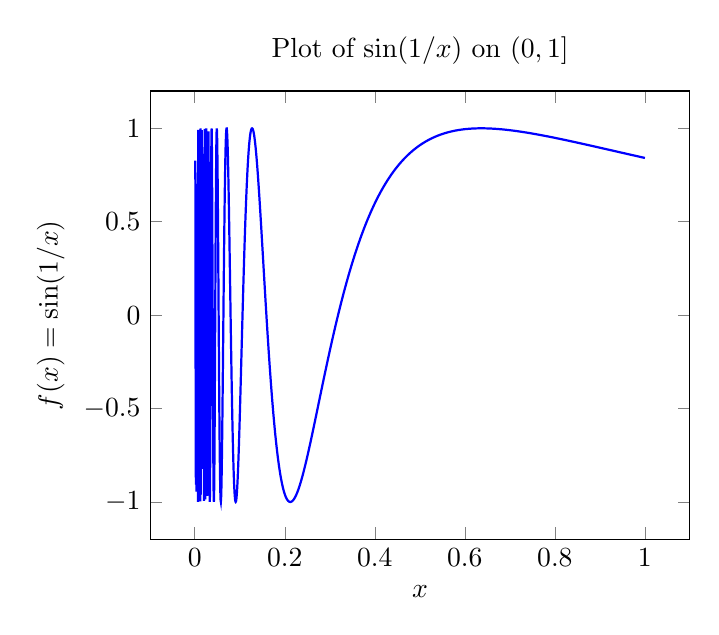
\begin{tikzpicture}
        \begin{axis}[
            domain=0.001:1,         % Domain from 0.01 to 1
            samples=2000,           % Number of sample points
            xlabel={$x$},          % Label for the x-axis
            ylabel={$f(x)=\sin(1/x)$}, % Label for the y-axis
            title={Plot of $\sin(1/x)$ on $(0,1]$}
          ]
          % Note: TikZ's sin function takes degrees by default,
          % so we convert 1/x from radians to degrees using deg(1/x)
          \addplot [blue, thick] {sin(deg(1/x))};
        \end{axis}
      \end{tikzpicture}

      $S$ is connected since it is the graph of a continuous function. Therefore, $\bar{S}$ is also.

      $\bar{S}=S \cup(\{0\} \times [-1,1])$

      Suppose there is a path between any point in $(\{0\} \times [-1,1])$ to a point in $SS$. $f:[a,b] \to \bar{S}$.

      Thus, $f^{-1}(\{0\} \times [-1,1])$ is a closed subset of $[a,b]$.

      Let $m = \sup f^{-1}(\{0\} \times [-1,1])$. This means that $f(m) \in \{0\} \times [-1,1]$.

      Can re-paramertize the interval $[m,b]$ to get a map

      $f:[0,1] \to \bar{S}$ satisfying:

      $f(0)=(0,y(0))$

      $f(t)=(x(t),y(t))$ where $x(t) > 0$ whenever $t>0$

      Find a sequence of times $t_n$ with $t_n \to 0$ s.t.

      $y(t_n)=(-1)^n$

      Given some $n$, can find some $u \in \R$ between $0$ and $x(1/n)$ s.t. $\sin(1/u)=(-1)^n$

      Since $x(t)$ is continuous, $x(1/u) > u$, $x(0)<u$. By the IVT then there is a $t_n \in [0,1/n]$ s.t. $x(t_n)=u$.

      This means that $y(t_n)=\sin(1/x(t_n))=\sin(1/u)=(-1)^n$

      Conclude that $t_n \to 0$, but $f(t_n)$ does not converge. Thus $f$ is not continuous.
}

\subsection{More on Connected Spaces}
\propp{
    Let $\{A_j\}_{j \in J}$ be a collection of connected subspaces of a space $X$. If $\displaystyle\bigcap_{j \in J}A_j$ is nonempty, then $\displaystyle\bigcup_{j \in J}A_j$ is connected.
}{
    Let $p \in \displaystyle\bigcap_{j \in J}A_j$m let $Y=\displaystyle\bigcup_{j \in J}A_j$.

    \noindent Suppose for contradiction that $Y$ is not connected. Then, there are open sets $C,D$ s.t. $Y=(C \cup Y) \cup (D \cap Y)$ and $C \cap Y$, $D \cap Y$ nonempty, disjoint.

    \noindent WLOG, $p \in C \cap Y$. Since each $A_j$ is connected and is a subspace of $Y$ we know that $A_j \subset C$ or $A_j \subset D$. But $p \in A_j \cap C$, so $A_j \subseteq C$ for all $j$.
    $Y \subset C$, so $Y \cap D = \emptyset$. $\contr$
}

\propp{
    Let $X,Y$ be connected spaces. Then $X \times Y$ is connected.
}{
    Fix $x \in X$. Then $\{x\} \times Y$ is homeomorphic to $Y$, so it's connected.

    \noindent For any $y \in Y$, the spaces $X \times \{y\}$ is connected.
    
    \noindent Let $T_y=(\{x\} \times Y) \cup (X \times \{Y\})$ be a subspace. It is connected since they intersect non trivially, and they are both connected.

    \noindent Since $X \times Y= \displaystyle \bigcup_{y\in Y}T_y$. But the intersection of all the $T_y$ is non-empty, so the unions is connected thus $X \times Y$ is connected.
}

\propp{
    Let $\{X_\alpha\}_{\alpha \in J}$ be a collection of connected spaces. Then $\displaystyle \prod_{\alpha \in J} X_\alpha$ is connected. (w/ product topology)
}{
    (in case where $\displaystyle \prod_{\alpha \in J} X_\alpha= \R^\omega$):

    \noindent Fix the point $(0,0,0,\dots) \in \R^\omega$.

    \noindent Given any $N$, define the subspaces $X_N \subseteq \R^\omega$ consisting of sequences $(x_n)$ satisfying $x_n=0$ for all $n > N$.

    \noindent $X_N$ is homeomorphic to $\R^N$. $X_N$ is connected since $\R^N$ is.

    \noindent $\displaystyle \bigcap_{N=1}^\infty X_N$ contains 0. Thus, the union is connected.

    \clmp{}{$\overline{\displaystyle\bigcup_{N=1}^\infty X_N}=\R^\omega$}{
        Let $U$ be any open set in $\R^\omega$, where $U=U_1 \times U_2 \times \dots \times U_n \times \R \times \R \times \dots$

        \noindent This open set $U$ intersect $\displaystyle_{N=1}^\infty X_N:$

        \noindent there is a point in $U$ of the form $(x_1,x_2,\dots,x_m,0,0,\dots)$

        \noindent This point lies in $X_M$. So every nonempty open set intersects the union, so its closure is $\R^\omega$ 
    }

    \noindent Thus since the closure of a connected space is connected $\R^\omega$ is connected.
}

\defn{Connected Component}{
    Let $X$ be a space. A connected component of $X$ is a maximal connected subspace of $X$. If $A$ is connected and $A \supseteq X$ and $A$ is connected, then $A=X$
}
\exm{}{
    $X=[0,1/2)\cup(1/2,1]$, each of $[0,1/2)$ and $(1/2,1]$ is a connected component.
}
Define an equivalence relation $\sim$ on $X$ by:

$x \sim y$ if there is a connected subspace of $X$ containing both $x$ and $y$.
\propp{
    Connected components are equivalence classes under $\sim$.
}{
    Every connected subspace of $X$ intersects exactly one equivalence class. If $C_1,C_2$ are equivalence class, and $x \in A \cap C_1$, $y \in A \cap C_2$ for connected set $A$, then $x \sim y$ so $C_1 = C_2$

    So, equivalence classes are connected:

    Fix $x_0 \in C$ for equivalence class $C$. For each $y \in C$ there is a connected $A_y$ containing $x_0,y$. Know $A_y \subseteq C$, so $\displaystyle\bigcup_{y \in C}A_c=C$.

    $\displaystyle\bigcap_{y \in C}A_y$ contains $x_0$ so $C$ is connected.

    If $A$ connected, contains equivalence class $C$, by def every $z \in A$ is equivalent to every $y \in C$, so $A \subseteq C$ and $A=C$.

    $X$ is connected $\iff$ $X$ has exactly one or zero connected components.
}
Connected components are closed, but not necessarily open.

\exm{}{
    Connected Components of $\Q$ are all singletons.
}
\defn{Totally Disconnected}{
    A space $X$ is totally disconnected if every point is a connected component.
}
\defn{Path Component}{
    Let $X$ be a space. A path component of $X$ is a maximal connected path of $X$. If $A$ is path and $A \supseteq X$ and $A$ is connected, then $A=X$
}